\documentclass[journal]{IEEEtran}

\ifCLASSINFOpdf
\else
   \usepackage[dvips]{graphicx}
\fi
\usepackage{url}

\usepackage{graphicx}
\usepackage{amsmath}
\usepackage{amssymb}
\usepackage{hyperref}  
\usepackage{float}
\usepackage{cuted}
\usepackage{graphicx}

\newtheorem{prop}{Proposition}
\newtheorem{thm}{Theorem}
\newtheorem{corol}{Corollary}
\newtheorem{proof}{Proof}


\begin{document}

\onecolumn

\section{Exact solution for multiple pre-synaptic inputs neuron unit}

\begin{figure}[h]
\centering
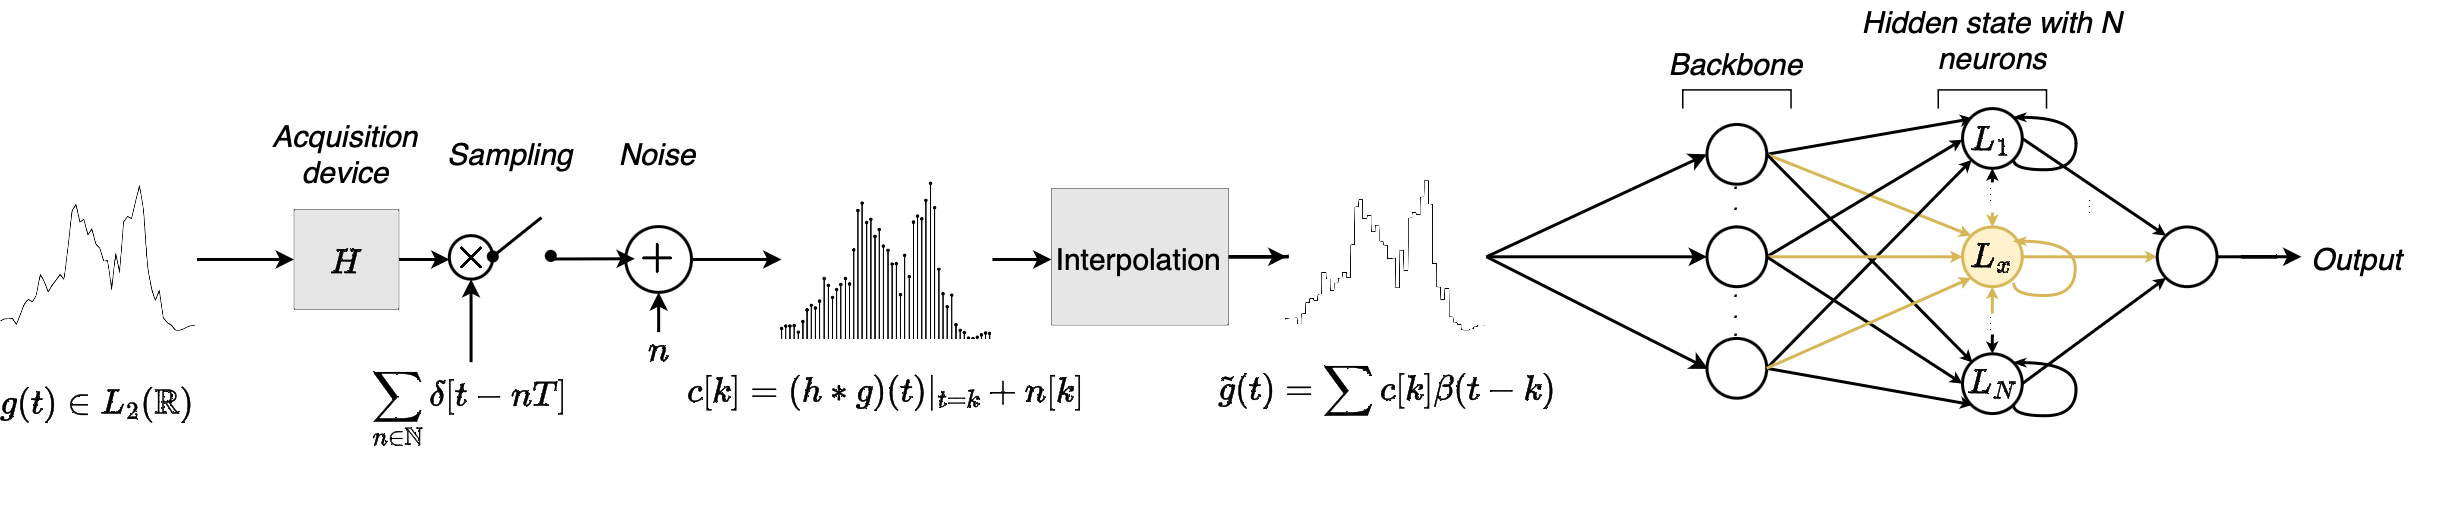
\includegraphics[width=1\textwidth]{general_pipeline.png} 
    \caption{ $L_2$-signal processing on the regular grid: a signal is convolved with the impulse response $h$ of an acquisition device $H$. Then it is regularly sampled where random noise $n[k]$ is added to the samples $c[k]$. The discrete sequence $c$ is then interpolated with a constant B-spline $\beta$ generator to represent a piecewise constant signal $\tilde y$ in the continuous domain. An intermediate layer $L$ of $N$ neurons is shown, where the highlighted neuron $L_x$ receives multiple pre-synaptic input signals.}
    \label{fig: General pipeline }
\end{figure}

\begin{figure}[h]
\centering
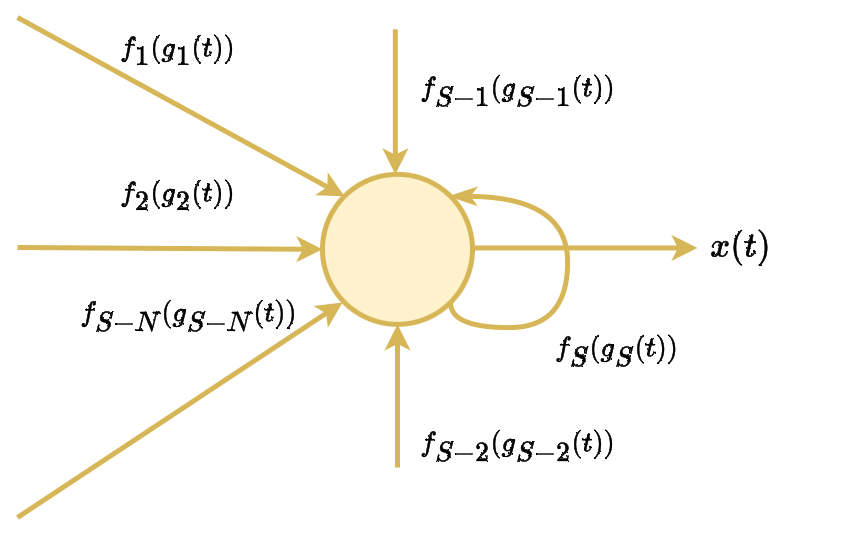
\includegraphics[width=0.5\textwidth]{unit.png} 
    \caption{Neuron units with multiple pre-synaptic inputs}
    \label{fig:units}
\end{figure}




We focus on the units of one neuron with multiple presynaptic stimulus as shown in the figure \ref{fig:units}.
Here, we will solve the neuron's dynamic equation involving a total number of $S$ synapses. The equation is derived as follow:
\begin{equation}
\frac{\mathrm{d}}{\mathrm{dt}}x(t)=-\omega x(t) + \sum_{s=0}^{S}f_s(\tilde{g}_s(t), \sigma_s, \mu_s)(A_s-x(t))
\label{eq: exact solution several synapses}
\end{equation}




For a total number of synapses $S$ containing input synapses from a previous layer and connecting synapses between neuron associated to a unique neuron, we have, for all \(s \in [1; S] \) and $t\in [\tau_k, \tau_{k+1}[$ :

$\tilde{g}_s(t) = c_s[k] \text{ : the pre-synaptic stimulus for synapse $s$}$

$f_s(t, \sigma_s, \mu_s) = f_s(t) = \frac{1}{1 - e^{-\sigma _s (t - \mu_s)}} \text{ : synaptic release non-linearity for synapse $s$}$
\vspace{1cm}

\textit{Theorem 1 :} : We compute the exact solution of \ref{eq: exact solution several synapses}, for piecewise constant input $\tilde{g} = (\tilde{g}_s)_{s\in [1, S]}$ and regularly or irregularly sampled inputs on time samples denoted by $(\tau_k)_{k\in \mathbb{N}} $  and $t\in [\tau_k, \tau_{k+1}[$:


\begin{equation}
 x(t) =  \alpha^{-1}(t) \left( x(0) + \Delta(t)\sum_{s=0}^{S} A_s u_s(\tau_i) +\sum_{i=0}^{k-1} \Delta(\tau_i)\sum_{s=0}^{S} A_s u_s(\tau_i) \right)
 \label{eq:exact solution}
\end{equation}
Where
\[
    u_s(\tau_i) = \frac{f_s(c_s[i])}{\omega + \sum_{\sigma=1}^{S}  f_{\sigma}(c_{\sigma}[i])}
\]
\[
    \alpha(t) = e^{\omega t + \sum_{s=0}^{S} (t-\tau_k)f_s(c_s[k])+\sum_{i=0}^{k-1}\sum_{s=0}^{S} (\tau_{i+1}-\tau_i)f_s(c_s[i])}
\]
\[
    \Delta(\tau_i) =\alpha(\tau_{i+1}) - \alpha(\tau_i)
\]
\[
    \Delta(t) =\alpha(t) - \alpha(\tau_k)
\]

\textit{Proof theorem 1 :}  


Let's denote 
\[
\beta_S(t) = \sum_{s=1}^S f_s(\tilde{g}_s(t))
\]
\[
c_S(t) = \sum_{s=1}^S A_s f_s(\tilde{g}_s(t))
\]

Equivalent problem:

\[
\frac{\mathrm{d}}{\mathrm{d}t} x(t)= - (\omega + \beta_S(t)) x (t) + c_S(t)
\]

Let's define:

\[
\alpha_S(t) = e^{\int_0^t (\omega+ \beta_S(u)) du} = e^{\omega t + \int_0^t \beta_S(u) du}
\]
\[
= e^{\omega t + \sum_{s=1}^{S} \int_{\tau_k}^{t} f_s(\tilde{g}_s(u))) du + \sum_{s=1}^{S} \sum_{i=0}^{k-1} \int_{\tau_i}^{\tau_{i+1}} f_s(\tilde{g}_s(u)) du} 
\]
\[
= 
e^{\omega t + \sum_{s=1}^{S} (t-\tau_k)f_s(c_s[k]) + \sum_{s=1}^{S} \sum_{i=0}^{k-1} (\tau_{i+1}-\tau_i)f_s(c_s[i])} 
\]
By multiplying by $\alpha_S$ the equation $(E)$, we get : 
\[
\alpha_S(t) \frac{\mathrm{d}}{\mathrm{d}t}x(t)  = -  (\omega + \beta_S(t)) \alpha_S(t) x (t) + c_S(t) \alpha_S(t)
\]

We observe that : 

\[
\alpha_S(t) \frac{\mathrm{d}}{\mathrm{d}t}x(t) + (\omega + \beta_S(t)) \alpha_S(t) x (t) = \frac{\mathrm{d} }{\mathrm{d}t}\alpha_S(t) x(t)
\]

Now we have:

\[
\alpha_S(t) x(t) = \int_0^t c_S(u) \alpha_S(u) du + C
\]

Let's find \(C\):

\[
\alpha_S(t = 0) = 1 \quad \Rightarrow \quad C = x (t = 0)
\]


\[
\alpha_S(t) x (t) - x (0) = \int_0^t c_S(u) \alpha_S(u) du
\]

Let's now compute \(\int_0^t c_S(u) \alpha_S(u) du\):



\[
\int_0^t c_S(u) \alpha_S(u) du = \int_0^t \sum_{s=1}^S A_s f_s(g_s(u))\alpha_S(u) du 
\]


\[
 = \sum_{s=1}^S A_s \int_0^t f_s(g_s(u))\alpha_S(u) du
\]
\[
 =  \sum_{s=1}^S A_s I_{S}(t, s)
\]


Let's now compute $I_{S}(t, s)$.




\[
 I_{S}(t,s) = \int_0^t f_s(\tilde{g}_s(u))\alpha_S(u) du
\]
\begin{multline*}
=\int_{\tau_k}^t  f_s(\tilde{g}_s(u))\alpha_S(u) du  + \sum_{i=0}^{k-1}\int_{\tau_i}^{\tau_{i+1} }f_s(\tilde{g}_s(u))\alpha_S(u) du 
\\
=\int_{\tau_k}^{t } f_s(\tilde{g}_s(u)) e^{\omega u + \int_0^u \beta_S(v) dv}du+ \sum_{i=0}^{k-1}\int_{\tau_i}^{\tau_{i+1} } f_s(\tilde{g}_s(u)) e^{\omega u + \int_0^u \beta_S(v) dv}du
\end{multline*}

As $u \in [\tau_i, \tau_{i+1}[$, we have :

\begin{multline*}
I_S(t, s)=\int_{\tau_k}^{t } f_s(c_s[k]) e^{\omega u + \sum_{s=1}^{S} (u-\tau_k)f_s(c_s[k]) + \sum_{s=1}^{S} \sum_{j=0}^{k-1} (\tau_{j+1}-\tau_j)f_s(c_s[j]) } du \\
+ \sum_{i=0}^{k-1} \int_{\tau_i}^{\tau_{i+1}} f_s(c_s[i]) e^{\omega u + \sum_{s=1}^{S} (u-\tau_i)f_s(c_s[i]) + \sum_{s=1}^{S} \sum_{j=0}^{i-1} (\tau_{j+1}-\tau_j)f_s(c_s[j])} du
\end{multline*}


\[
 = f_s(c_s[k]) \frac{e^{\omega t + \int_0^t\beta_S(u)du } - e^{\omega \tau_k + \int_0^{\tau_k}\beta_S(u)du  }}{\omega + \sum_{\sigma = 1}^{S}f_\sigma(c_{\sigma}[k]) } +\sum_{i=0}^{k-1} f_s(c_s[i]) \frac{e^{\omega\tau_{i+1}+ \int_0^{\tau_{i+1}}\beta_S(u)du}- e^{\omega \tau_i +  \int_0^{\tau_{i}}\beta_S(u)du}}{\omega + \sum_{\sigma = 1}^{S}f_\sigma(c_{\sigma}[i])}
\]


Then the final expression for the neuron's dynamic is the following :

\begin{multline*}
 x(t)=  (x(0) + \sum_{s=1}^S A_s( f_s(c_s[k]) \frac{e^{\omega t + \int_0^t\beta_S(u)du } - e^{\omega \tau_k + \int_0^{\tau_k}\beta_S(u)du  }}{\omega + \sum_{\sigma = 1}^{S}f_\sigma(c_{\sigma}[k]) }\\ +\sum_{i=0}^{k-1} f_s(c_s[i]) \frac{e^{\omega\tau_{i+1}+ \int_0^{\tau_{i+1}}\beta_S(u)du}- e^{\omega \tau_i +  \int_0^{\tau_{i}}\beta_S(u)du}}{\omega + \sum_{\sigma = 1}^{S}f_\sigma(c_{\sigma}[i])}) ) e^{- \omega t - \int_0^t \beta_S(u) du}
\end{multline*}




\[
 x(t)=  (x(0) + \sum_{s=1}^S A_sf_s(c_s[k]) \frac{\alpha(t)-\alpha(\tau_k)}{\omega + \beta_S[\tau_k]} + \sum_{s=1}^S\sum_{i=0}^{k-1} A_sf_s(c_s[i]) \frac{\alpha(\tau_{i+1})-\alpha(\tau_i) }{\omega + \beta_S(\tau_i)})\alpha^{-1}(t)
\]



To simplify the given expression for \( x(t) \):


\[
 x(t) = \alpha^{-1}(t) \left( x(0) + \left(\alpha(t) - \alpha(\tau_{i})\right) \sum_{s=0}^{S} A_s u_s(\tau_i)  + \sum_{i=0}^{k-1} \left(\alpha(\tau_{i+1}) - \alpha(\tau_{i})\right) \sum_{s=0}^{S} A_s u_s(\tau_i) )\right)
\]
\[
 = \alpha^{-1}(t) \left( x(0) + \Delta(t)\sum_{s=0}^{S} A_s u_s(\tau_i) +\sum_{i=0}^{k-1} \Delta(\tau_i)\sum_{s=0}^{S} A_s u_s(\tau_i) \right)
\]


\textit{Corollary 1 : } We do observe a recursive relationship between $\tau_{k+1}$ and $\tau_{k}$ :

\[ x(\tau_{k+1})
 = e^{-\omega(\tau_{k+1}-\tau_k) - \sum_{s=0}^{S}(\tau_{k+1}-\tau_{k})f_s(c_s[k]))} \left(x(\tau_{k}) -\sum_{s=0}^{S} A_s w_s(\tau_{k})\right) + \sum_{s=0}^{S} A_s w_s(\tau_{k})
\]

\textit{Proof corollary 1 : }

\[
 x(\tau_{k+1})= 
 \alpha^{-1}(\tau_{k+1}) \left( x(0) + \sum_{i=0}^{k} \Delta(\tau_i)  \sum_{s=0}^{S} A_s w_s(\tau_i) \right) 
\]

\[
 = \alpha^{-1}(\tau_{k+1})\left(\alpha(\tau_{k}) x(\tau_{k}) + \Delta(\tau_{k})  \sum_{s=0}^{S} A_s w_s(\tau_{k})\right)
\]
\[
 = \alpha^{-1}(\tau_{k+1})\alpha(\tau_{k}) \left(x(\tau_{k}) -\sum_{s=0}^{S} A_s w_s(\tau_{k})\right)) + \sum_{s=0}^{S} A_s w_s(\tau_{k})
\]
\end{document}

